% sections/evidence.tex: Section 3, what the tests of the advice found (one outcome metric: the rank-based citation score
% of the one-change-at-a-time tests, CE/experiments/RESULTS_E1.md, CE/experiments/RESULTS_E2.md, CE/experiments/RESULTS_E3.md).
% Draft 2, 2026-10-24: cut from about 1,430 to about 640 words to fit 4 pages (notes/CUTS.md).
% Clarity pass, 2026-10-26 (notes/CLARITY-PASS.md): prose cut from about 540 to about 360 words. The laptop bench (word share) and the
% sensitivity test (citation share) are one sentence each, as context; method detail is one sentence plus the Research
% page; results name checks, not experiment arms; numbers that Figure 4 shows were dropped from the text. The nine
% sources' citations moved to Section 2.1 (sec:checks).
%   CE     = ../citation-equity (tool repo, read only; numbers first checked at commit f38d34e, src pointers rechecked
%            at the feat head c908431 on 2026-10-26; public main b10887e has the same files except CE/docs/superpowers and CE/docs/research/*.json)
%   S-JSON = CE/experiments/results/sensitivity/sensitivity_{Qwen__Qwen3.5-9B, google__gemma-4-12B-it,
%            Qwen__Qwen3.8-27B, google__gemma-4-31B-it}.json
% Every number carries a "% src:" comment. Derived numbers cite data/sensitivity_derived.json (scripts/derive_sensitivity.py).
% "E1", "E2" and "E3" are named only in comments (and once in the E4 owner mark); the prose says "our first test" and
% "follow-up tests".

\section{What the tests found}\label{sec:evidence}\label{sec:findings}

% src: CE/samples/README.md lines 43 to 50 ("The first recording, and why it was superseded"; CE c908431): 4,096-token default window,
%      prompts about 3,500 tokens, 3 truncated calls; 13 of 128 answers without a valid [n]; no chance level reported
% src: p floor: CE/samples/README.md line 98 ("With 4 questions the smallest possible p is 0.125, so these runs can show a direction
%      at most.")
% src: CE/samples/README.md lines 81 and 87 to 98 (llama3.2:3b, 128 answers all valid; 5.3 to 6.5 of 8 sources cited;
%      word share 0.087 -> 0.137 and 0.086 -> 0.095; chance 0.125 inside every 95% interval; paired p 0.25 and 0.75,
%      smallest possible 0.125)
On the authors' laptop the bench shows a direction at most: every 95\% interval of the draft's word share included the 0.125 chance level, $p \geq 0.125$ with 4 questions, and a first recording, misread through truncated prompts, was withdrawn.
% src: CE/experiments/RESULTS_sensitivity.md and data/sensitivity_derived.json (unchanged from draft 2): 4 models x 256
%      valid answers, 8 questions x 8 seeds, 7 synthetic competitors, no retrieval; plan 3c86c02 before results 4d77fa0
%      (CE/experiments/PREREG_sensitivity.md, "Criteria (fixed before running)"); answer edit +0.007 to +0.034 vs bar
%      +0.10, detectable difference for the answer edit (mde_post_hoc of answer_first_minus_before) 0.019 to 0.047, below
%      the bar (data/sensitivity_derived.json "ranges"."mde_post_hoc_answer_first"); after draft +0.014 to +0.031;
%      drafts 14% and 22% longer (`wc -w` on CE/samples/*/{before,after}.md, rechecked 2026-10-26: 831 -> 946 and
%      1,041 -> 1,275); off-topic control <= 0.0031 (shown in Figure 1b)
A sensitivity test planned in advance, with four open models and synthetic competitors, measured \emph{citation share}: a one-sentence answer edit gained only $+0.007$ to $+0.034$ against a $+0.10$ target the harness could detect, and the full after drafts, 14\% and 22\% longer, gained $+0.014$ to $+0.031$ (Figure~\ref{fig:overview}b).

\paragraph{One change at a time.}
% src: CE/experiments/PREREG_E1.md (frozen r3 at 7859b07, before any page was edited; amendments 1-10 at its end) and
%      CE/experiments/RESULTS_E1.md (commit e258a1a; data/e1_results.json): 80 main queries (GEO-bench test split,
%      informational), 60 C-SEO Bench queries; editor Gemma-4-31B-it edits only the flagged spans, validators reject edits
%      that add facts or miss the check; reference = a same-length paraphrase of the same spans; 4 sources per prompt, slot
%      rotated; judges Gemma-4-12B-it and Qwen3.8-27B, 8 seeds; score (5 - r)/4 with r = 5 if uncited
%      (CE/experiments/PREREG_E1.md line 119); 17,823 of 17,824 answers valid (CE/experiments/e1/out/score_summary.json);
%      plans for the follow-ups: CE/experiments/PLAN_E2.md line 3 and CE/experiments/PLAN_E3.md line 3
% src: Research page https://shehral.github.io/citation-equity/research/ (HTTP 200 on 2026-10-26; reports E1 to E3 with
%      Holm-adjusted results), listed with the code and data in the intro footnote (fn:links)
Our first test applies one check's suggestion alone to real pages (80 informational GEO-bench queries~\cite{aggarwal2024geo}, replicated on 60 from C-SEO Bench~\cite{puerto2025cseo}): an open model edits only the spans the check flags, and each edit is compared with a same-length paraphrase of those spans; two open judges see the page among 4 sources, and its \emph{citation score} is $(5-r)/4$ when it is the $r$-th source cited, else 0 (plans fixed in advance, code and data: footnote~\ref{fn:links}).

% src: CE/experiments/RESULTS_E1.md main primary contrasts: arm 9 (target questions answered, done as a section headed by
%      the question) +0.027 [+0.010, +0.043] Holm 0.006 n 54, replication +0.036 n 52; arm 12 (query words in title and
%      lead = the reader's-words check) +0.035 [+0.008, +0.066] Holm 0.037 n 33; confound-adjusted intercepts include 0
%      (arm 9 [-0.075, +0.018], arm 12 [-0.083, +0.018], ALL-original [-0.012, +0.096]); data/e1_results.json "main",
%      "replication"; all fixes (ALL +0.049 n 78, +0.071 vs P_ALL n 53, replication +0.044) are shown in Figure 4 only
Of single changes, only the two that add the reader's own words near the top clearly raised the score (Figure~\ref{fig:e1}): \emph{target questions answered}, done as a section headed by the question ($+0.027$, 95\% CI $[+0.010, +0.043]$, Holm $p = 0.006$; replication $+0.036$), and \emph{your reader's words up top}, the question's missing words in title and lead ($+0.035$); for both, the effect left after regressing out length and question-word changes includes zero.
% src: CE/experiments/RESULTS_E2.md, E2a planned tests (d = arm 9 minus 9W or 9P; data/e1_results.json "e2"."e2a"):
%      9 vs 9W main +0.003 [-0.009, +0.016] n 54, replication -0.001 [-0.014, +0.012] n 52, both "no effect larger
%      than delta"; 9 vs 9P replication +0.048 [+0.027, +0.071] Holm p < 0.001 "helps", main +0.017 [+0.001, +0.033]
%      Holm 0.089 "inconclusive" (both shown in Figure 4 only; the text no longer states them); reported without a verdict: 9W vs original +0.023 (main) and
%      +0.037 (replication)
Follow-up tests, each planned before its answers, place the gain in the words, not the form: the question heading did no better than the same text set as plain ($+0.003$; replication $-0.001$) while the plain-text question scored higher than the untouched page ($+0.023$; $+0.037$).
% src: CE/experiments/RESULTS_E2.md, E2b (editor Qwen3.8-27B; judges Gemma-4-12B and Qwen3.5-9B; data/e1_results.json
%      "e2"."e2b"): 12 vs P12 +0.029 [+0.003, +0.061] n 29; ALL vs P_ALL +0.069 [+0.038, +0.104] n 44; both keep E1's sign
With another editor and other judges, the reader's-words gain kept its sign ($+0.029$, $n = 29$), as did all fixes together ($+0.069$, $n = 44$).
% src: CE/experiments/RESULTS_E3.md "Pooled result" (data/e1_results.json "e3"; 260 queries, 180 new): arm 2 -0.016
%      n 57, arm 7 -0.010 n 49, arm 8 +0.012 n 66 "no effect larger than delta"; arm 6 +0.026 [+0.001, +0.053] n 62
%      Holm 0.179 "inconclusive"; arms 4, 5, 10 n 11, 11, 24 (all shown in Figure 4); "Where the queries come from"
%      (E1's queries gained at most 4 pairs from the extra attempt; the editor runs at temperature 0,
%      CE/experiments/PREREG_E1.md line 85); lists: E1 arm 3 -0.007 n 33 "no effect larger than delta" (RESULTS_E1.md)
A second follow-up added 180 queries for the checks with too few pages: over 260, question headings, cited sources and direct answer first showed no effect larger than 0.03 and attributed quotes were inconclusive; tables, statistics and comparisons still had too few.
% The owner approved this tool update (task brief, 2026-10-24). The rule's outcome (four unscored notes, the new reader's-words
% check) is stated once, in Section 2.1 (sec:checks); the sentence that repeated it here was cut (notes/CUTS.md 68).
% src for that outcome: CE commits 27201da (reader-words check), 8219c90 (measured fixes first) and 00d65b7 (E3's pooled
%      results; question headings, cited sources, direct answer first unscored), merged at 4831ff9; CE/docs/evidence.md line 34 (CE c908431)
% Reserved space (clarity pass 2026-10-26): about 4 lines for the Gemini judge check of the three key comparisons; the
% build was checked with 4 lines of filler here (notes/CLARITY-PASS.md).
% E4 (a Gemini judge check) was stopped before analysis on 2026-10-26 (free-tier quota); see CE/experiments/PLAN_E4.md. Nothing reported.

% ---------------------------------------------------------------------------------------------------------------
\begin{figure}[t]
  \centering
  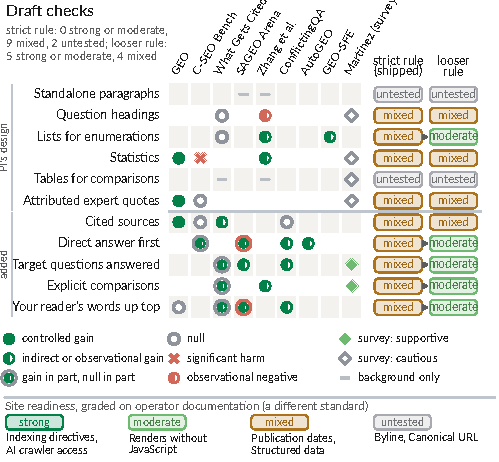
\includegraphics[width=\columnwidth]{figures/fig3_evidence.pdf}
  \Description{A matrix with the eleven draft checks as rows and the nine sources as columns. Each cell marks a controlled gain, an indirect or observational gain, a gain in part with a null in part, a null, a significant harm, an observational negative, survey support or caution, or background only. Two chip columns give each check's grade under the strict shipped rule (9 mixed, 2 untested) and under a looser rule (5 moderate, 4 mixed, 2 untested). A strip below grades the seven site-readiness items.}
  % src (caption): CE/docs/evidence.md line 34; data/evidence_grades_loose.json tally (strict 0/0/9/2; loose 0/5/4/2);
  %      readiness_tally 2 strong, 1 moderate, 2 mixed, 2 untested; single-rater coding (data/README.md)
  % cite order in the caption = the columns, left to right (moved from Section 3's "The grades" in the clarity pass)
  % columns, left to right, follow scripts/figdata.py STUDIES (CE/docs/evidence.md table rows at lines 80 to 88); rows follow the
  %      engine registry (eleven checks; reader's words last, coded from CE/docs/evidence.md lines 255 to 258); cell lines in
  %      data/evidence_matrix.csv remapped to CE c908431 on 2026-10-26 (+2 after line 37, identical text)
  \caption{\figtakeaway{Every tested draft check has a null or negative result somewhere, but ``mixed'' spans positive-in-every-model to harmful, and a looser rule, defined post hoc, moves five to moderate.}
    Columns: \cite{aggarwal2024geo}, \cite{puerto2025cseo}, \cite{vishwakarma2026cited}, \cite{kim2026sageo}, \cite{zhang2026absorption}, \cite{wan2024conflictingqa}, \cite{wu2026autogeo}, \cite{yu2026geosfe}, \cite{martinez2026survey}. One rater.}
  \label{fig:evidence}
\end{figure}

\begin{figure}[t]
  \centering
  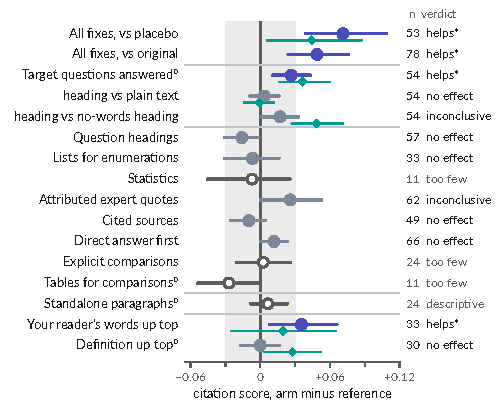
\includegraphics[width=\columnwidth]{figures/fig4_e1.pdf}
  \Description{A forest plot over real web pages. Each row is one check's suggestion applied alone, or all fixes together, with the mean difference in citation score from its reference and a 95 percent interval, a shaded band from minus 0.03 to plus 0.03, and small teal diamonds for the 60-query replication. All fixes together, target questions answered and your reader's words up top sit to the right of the band. Two rows under target questions answered compare its question heading with the same text as plain text (near zero) and with a heading without the question's words (positive, clearly so in the replication). Question headings, lists, cited sources and direct answer first sit inside the band; attributed expert quotes is inconclusive; statistics, explicit comparisons and tables for comparisons have open circles with too few pages.}
  % src (caption): data/e1_results.json ("main", "replication", "e2", "e3"); scripts/fig_e1.py (row names = Figure 3's check names)
  % Clarity pass: "260 queries for question headings and statistics to tables, 80 for the rest" dropped (Section 3 says which
  % checks the 260-query follow-up covers; notes/CUTS.md 79).
  \caption{\figtakeaway{Of single changes, only the two adding the reader's words up top clearly raised citation; the heading form, sources and answer-first showed no effect larger than 0.03; quotes were inconclusive.}
    Difference from a same-length paraphrase or the original ($^{\circ}$), 95\% intervals; filled: 30+ pages; band: $\pm 0.03$; teal: replication; helps$^{*}$: possibly via question-word overlap.}
  \label{fig:e1}
\end{figure}

\begin{figure}[t]
  \centering
  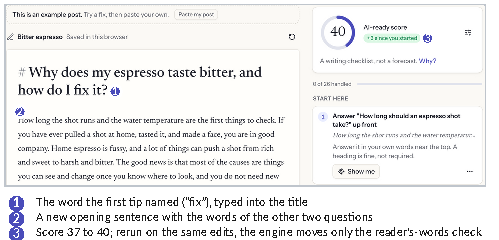
\includegraphics[width=\columnwidth]{figures/fig5_reader_words.pdf}
  \Description{A screenshot of the deployed draft view on the espresso example after two edits. Left: the title now reads "Why does my espresso taste bitter, and how do I fix it?" and the first paragraph opens with "How long the shot runs and the water temperature are the first things to check." Right: the AI-ready score of 40 with a green chip "+3 since you started", the line "A writing checklist, not a forecast", and the first Start-here fix. Numbered callouts mark the title words, the opening sentence and the chip.}
  % src (caption): data/fig5_callouts.json (scripts/capture_reader_words.mjs, live site 2026-10-26): score_before "AI-ready
  %      score: 37 out of 100", score_after "... 40 out of 100", chip "+3 since you started", tips read before each edit
  %      (first: Add "fix"; second: Add "long"; none left after the opening sentence); "engine" block: the tool repo engine
  %      (CE c908431) on CE/samples/espresso-bitterness/before.md and the same two edits, the four sample questions as
  %      questions and reader's questions: Standard 37 -> 40, only reader-words changed (0.667 -> 1.000)
  \caption{\figtakeaway{Following the reader's-words tips raises the score: the tool now scores what helped.}}
  \label{fig:readerwords}
\end{figure}
